\section{Git and GitHub}
In this project, we use GitHub to host our project report LaTeX code and the source code for our Flutter application.
We use Git to interact with GitHub and push and pull code. 

GitHub is linked to our Azure Pipelines as described in~\autoref{azurepipelines}.

We use the principles of GitFlow, that requires developers to create a branch for each new feature, hotfixes and bug fixes. 
The branches can then be merged back into their respective branches when the implementation is completed.
This is done using pull requests, which have to be approved by at least one other developer enforcing a higher standard of code.

\begin{figure}[H]
    \centering
    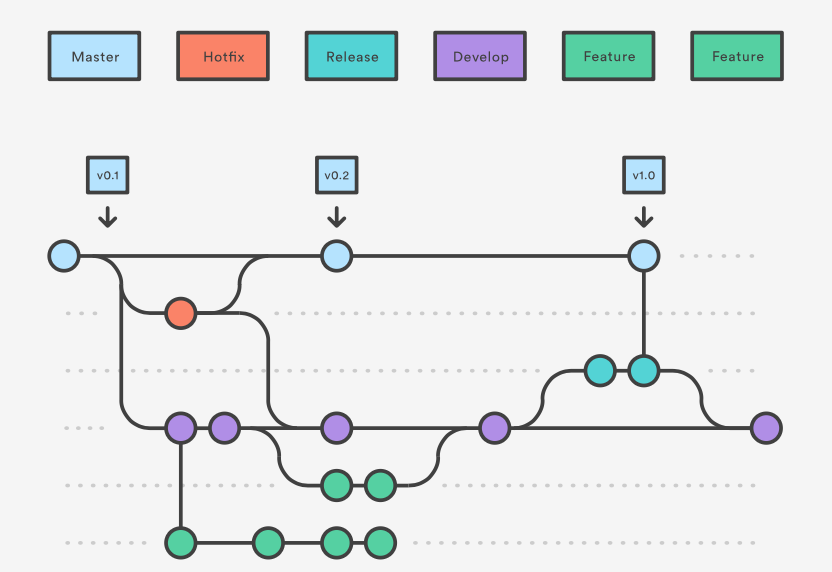
\includegraphics[width=0.8\textwidth]{images/GitFlow.png}
    \caption{GitFlow diagram, showing how branches should be created and named~\cite{GitFlowAtlassian}.}
    \label{Gitflow}
\end{figure}

\subsection{Git and GitHub within the Application}
As software developers ourselves, we have experience using GitHub.
However, some Product Owners will have very limited or no experience at all with either Git or GitHub.
We thought if the issues could be made directly by the Product Owner, it would make it easier for the developers to focus on working on the issues instead of creating and managing issues. 
Our solution allows any Product Owner with no Git or GitHub experience, to create issues and tasks which developers already know how to use.
Our application also allows the Product Owner to see communication between developers, and intervene and make sure that the developers are on track.

Since the application is already integrated with GitHub it was easy to implement a way for the Product Owner to be updated on the progress without the developers having to actively do so.
This is done by having the developer update the labels on the issue on GitHub, and the results in the application showing the status of the different issues. 

In this project, we only implemented GitHub, since it is something we are very familiar with, but any alternative to GitHub such as BitBucket, Phabricator, GitLab, Atlassian, SourceForge or Launchpad, etc. would work just as well.
However, they each would require a specific implementation to be supported.
Such an implementation would likely be trivial, by changing the API and endpoints, which does not require a lot of implementation, but for our MVP GitHub is enough as a proof of concept.
This is because all these products all use the notion of issues to keep track of tasks within a project.